\subsection{Sobre Cross Validation con K-Fold}

Como fue propuesto por la cátedra, para validar que la elección de nuestros parámetros para el sistema lleven luego a una buena generalización al momento de clasificar dígitos, utilizamos la técnica de cross validation con K-Fold.

¿En qué consiste? Para el caso de KNN+PCA, por ejemplo, tenemos que elegir entre $(k_i, \alpha_i)$ óptimos, por lo que para cada par se partirá el trainset disponible en $K$ conjuntos para luego hacer $K$ pruebas, donde en cada una de ellas la unión de $K-1$ conjuntos pasan a ser un nuevo trainset y el restante pasa a ser un nuevo testset. Al menos cada conjunto fue un testset después de haber aplicado K-Fold. Luego, promediando algúna métrica de performance entre las $K$ disponibles se puede obtener el valor final para la misma, la cual puede ser comparada después con las generadas por otros pares de hiperparámetros. Los elegidos van a poder ser validados con el testset original.

Las preguntas que se listan a continuación surgieron de pensar las cosas mencionadas en el párrafo anterior y se realizaron pruebas teniendo en cuenta los siguientes atributos:

\begin{itemize}
    \item \textbf{Métrica de performance}: Accuracy, tomando la media.
    \item \textbf{Algoritmo}: KNN+PCA
    \item \textbf{Rango de $K$}: $\{5, 10, 15, 20\}$
    \item \textbf{Rango de $k$}: $\{1\dots51, 5\}$
    \item \textbf{Rango de $\alpha$}: $\{10\dots100, 10\}$
    \item \textbf{Dataset}: Primeros 10000 elementos del dataset original, tomando el $80\%$ como trainset y el restante como testset.
\end{itemize}

\subsubsection{¿Qué valor debería tener K?}\label{KFoldValueK}

Elegir los hiperparámetros con validación simple consiste en hacer $n$ corridas de nuestro sistema, donde $n$ es el número de hiperparámetros candidatos que tenemos. Hacerlo con cross validation utilizando K-Fold nos lleva a realizar $n * K$ corridas del sistema, por lo que el tiempo de duración del experimento puede llegar a ser grande. Dependiendo de, entre otras cosas, el tamaño del dataset y la eficiencia general de los algoritmos.

Esto nos llevó a probar inicialmente con una serie de valores fijos para $K$ y una parte del dataset original para ver si, la métrica de performance variaba mucho, e inferir en ese caso si vale el costo temporal o no hacer la validación con valores de $K$ cada vez más altos.

\begin{itemize}
    \item \textbf{Pregunta}: ¿Será apreciable la variación de nuestra métrica de performance si K crece?
    \item \textbf{Hipótesis}: Si: Agregar K-Fold permitiría ver como se comporta el sistema con $K$ trainsets distintos, por lo que es factible que mientras más trainsets existan, se van a poder elegir hiperparámetros que generalicen mejor y maximicen la métrica de performance.
\end{itemize}

\subsubsection*{Análisis y resultado}

Los mejores hiperparámetros obtenidos fueron $(k = 1, \alpha = 40)$

\begin{figure}[H]
    \centering
    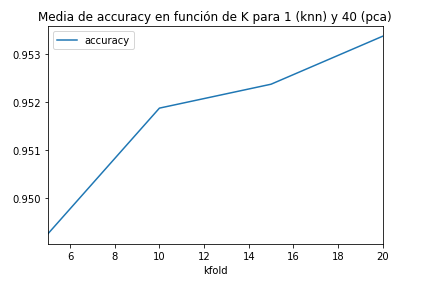
\includegraphics[scale=0.7]{images/KFoldIncreasingK.png}
    \caption{Cambios en el accuracy para un trainset de 8000 elementos en función de $K$ para K-Fold}
    \label{fig:KFoldIncreasingK}
\end{figure}

Como se puede apreciar en la figura \ref{fig:KFoldIncreasingK}, efectivamente, hubo una mejora en el accuracy, aunque parece no ser significativa para el tiempo demandado. Esto quedará más claro cuando se analice el mismo.

A juzgar por esta prueba queda claro que mientras mayor sea $K$, mayor es el accuracy por lo que es más conveniente, al menos tomar $K = 20$.

\subsubsection{¿Qué relación hay entre K y el tamaño del trainset?}

Esta pregunta tiene al menos dos aristas: desde la perspectiva del tiempo demandado y desde la perspectiva de la métrica de performance.

Es lógico pensar que a mayor tamaño del trainset, mejor podría generalizar un sistema para hiperparámetros dados, lo que lleva a pensar también que de hacer cross validation con K-Fold, por lo mencionado en la subsección anterior, puede demandar más tiempo.

Para las siguientes pruebas, el trainset definido de 8000 elementos, lo particionamos en cuatro trainsets: el primero de 2000, el segundo de 4000, el tercero de 6000 y el último (el completo) de 8000 elementos.

\subsubsection*{Desde la perspectiva de nuestra métrica de performance}\label{KFoldTrainSizeAcc}

\begin{itemize}
    \item \textbf{Pregunta}: A mayor tamaño del trainset y de $K$, ¿el accuracy también será mayor?
    \item \textbf{Hipótesis}: Si: de alguna forma será mayor en proporción a la cantidad de elementos que haya en el conjunto de entrenamiento. De esta forma, la mejor elección de nuestros hiperparámetros la vamos a poder realizar con el dataset completo (42000 elementos) propuesto por la cátedra.
\end{itemize}

\subsubsection*{Análisis y resultado}

Para los mismos hiperparámetros obtenidos, la evaluación fue consistente con la hipótesis planteada:

\begin{figure}[H]
    \centering
    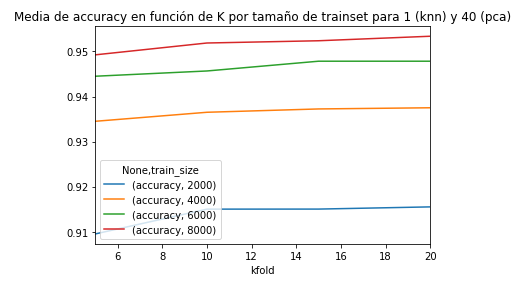
\includegraphics[scale=0.7]{images/KFoldAccTrainSize.png}
    \caption{Cambios en el accuracy para trainsets de diferentes tamaños en función de $K$ para K-Fold}
    \label{fig:KFoldAccTrainSize}
\end{figure}

En la figura \ref{fig:KFoldAccTrainSize} se puede observar, análogamente al caso anterior que para diferentes tamaños de trainset se ven pequeñas mejoras a medida que aumenta el valor de $K$, pero la diferencia notable en el accuracy está precisamente en el tamaño de mencionado conjunto. Aunque también es llamativo ver que la diferencia de la métrica entre el conjunto de 4000 y el de 2000 elementos es mayor a la que hay entre el conjunto de 6000 y 4000 elementos, y a su vez esta es mayor a la diferencia entre el conjunto de 8000 y el de 6000 elementos, lo que nos lleva a pensar que hay un límite para la mejora por el tamaño del trainset y que entrenar nuestro sistema con el dataset completo (42000 * 0.8) puede dejar esta métrica cercano a él.

\subsubsection*{Desde la perspectiva del tiempo demandado}\label{KFoldTrainSizeDuration}

\begin{itemize}
    \item \textbf{Pregunta}: A mayor tamaño del trainset y de $K$, ¿el tiempo demandado será mayor?
    \item \textbf{Hipótesis}: Si: de alguna forma será mayor en proporción a la cantidad de elementos que haya en el conjunto de entrenamiento. De esta forma, la búsqueda con el dataset completo de la mejor elección de nuestros hiperparámetros puede demorar sustancialmente.
\end{itemize}

\subsubsection*{Análisis y resultado}

Para los mismos hiperparámetros obtenidos, la evaluación no fue consistente con la hipótesis planteada:

\begin{figure}[H]
    \centering
    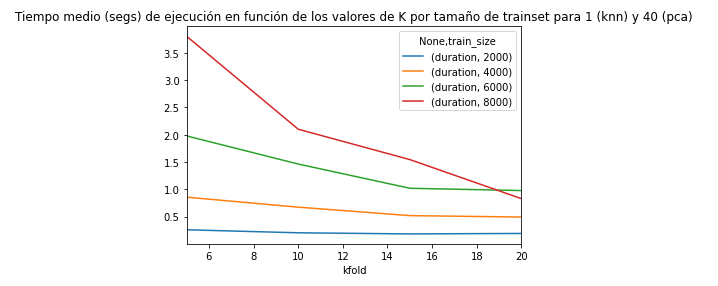
\includegraphics[scale=0.7]{images/KFoldDurationTrainSize.png}
    \caption{Duración media en segundos por tamaño de trainset para hiperparámetros encontrados: Se puede ver una disminución en el tiempo de ejecución a medida que aumenta $K$.}
    \label{fig:KFoldDurationTrainSize}
\end{figure}

Contra nuestra intuición, se puede ver en la figura \ref{fig:KFoldDurationTrainSize} una disminución en el tiempo de ejecución a medida que aumenta $K$ por un lado, la que se muestra más pronunciada a medida que aumenta el tamaño del trainset. Es interesante notar que por ejemplo para el conjunto de 8000 elementos si se realiza K-Fold con $K=5$ demora casi tres veces más que realizarlo con $K=20$. 

¿Por qué es así?: Supongamos dos casos:

\begin{itemize}
    \item \textbf{Trainset de 8000 elementos y $K=5$}: Cada instancia de entrenamiento tendrá un total de 6400 elementos y la de validación 1600. Para KNN se harán aproximadamente 10 millones de comparaciones terminar la clasificación.
    \item \textbf{Trainset de 8000 elementos y $K=20$}: Cada instancia de entrenamiento tendrá un total de 7600 elementos y la de validación 400: Para KNN se harán aproximadamente 3 millones de comparaciones terminar la clasificación.
\end{itemize}

Lo mencionado es en base a nuestra implementación de KNN, la cual es simple y para cada elemento que se quiera validar, se calculará la distancia con todos aquellos que se utilizaron para entrenar.

Al tomar la media de los tiempos para cada caso, se divide por $K$, por lo que en el caso $K=5$ no solo tenemos un tiempo grande, si no que lo estamos dividiendo por un número chico, contrariamente a lo que pasa con $K=20$.

\subsubsection{¿Conviene utilizar K-Fold? ¿Cuándo no?}

Utilizar K-Fold nos resulta útil para elegir los hiperparámetros con cierta confianza de que no van a haber mayores problemas generalizando a datos desconocidos. A cambio permitimos que la información se reorganice en cada prueba de diferentes maneras. Eso mismo puede ser prohibitivo para modelos en los que haya una componente temporal presente, dado que se pierde el sentido en la data.

\subsubsection{Finalmente: ¿qué valor debería tener K?}

Vimos en la subsección \ref{KFoldValueK} que podriamos tomar $K=20$, dado que a mayor $K$, mayor accuracy. Pero también comentamos que el aumento no parecia ser significativo para el tiempo demorado.

En \ref{KFoldTrainSizeAcc} vimos que la mayor confianza se obtiene cuando el trainset tiene un tamaño grande, mientras más mejor.

Contra intuitivamente, pensamos en también en \ref{KFoldTrainSizeDuration} que aumentar el tamaño del mismo podía llevarnos a requerir más tiempo para hacer la validación, lo que resultó no siendo cierto. No obstante el resultado lo vimos para una instancia de $(k, \alpha)$ y aunque la tendencia es cierta para cualquier combianción de ellos, la suma total de todo el tiempo necesario para probar las combinaciones de esas dos variables, con un dataset completo (42000 elementos) puede ser equivalente a toda una noche de ejecución. A modo de ejemplo, las pruebas de esta sección totalizarón un total de aproximadamente 3hs de ejecución en serie.

Por esta razón decidimos obviamente maximizar tanto como se pueda (y pide el enunciado) el tamaño del trainset y compensar eligiendo $K=10$, más intermedio para hacer las pruebas.